\chapter{Apresentação do Protótipo Funcional}
\label{cha:funcionalidades}

Este capítulo apresenta a materialização do sistema ViaBus através de seu protótipo funcional de \textit{frontend}. O objetivo aqui não é apenas exibir as telas desenvolvidas, mas demonstrar como as funcionalidades implementadas atendem diretamente aos Requisitos Funcionais (RF) definidos no Capítulo~\ref{cha:requisitos}, solucionando os problemas operacionais identificados na pesquisa de mercado.

A interface foi desenvolvida seguindo os princípios de usabilidade e \textit{design} responsivo (RNF01, RNF02), garantindo uma experiência de usuário clara e consistente em diferentes dispositivos. As seções a seguir estão organizadas de acordo com o fluxo de trabalho de um gestor: o \textit{onboarding} inicial, o gerenciamento dos recursos da empresa e, por fim, a execução das operações diárias.

\section{Onboarding e Visão Geral do Sistema}

A primeira interação do usuário com o sistema envolve a autenticação e o acesso ao painel de controle, que fornece uma visão geral das operações.

\subsubsection{Autenticação e Criação de Empresa}
Para garantir a segurança e o isolamento dos dados (RNF05, RNF06), o sistema implementa um fluxo de autenticação via e-mail e senha, gerenciado pelo NextAuth, conforme visto na Figura~\ref{fig:tela-login}. No primeiro acesso, o usuário é guiado por um formulário para cadastrar os dados de sua empresa (Figura~\ref{fig:criacao-empresa}), estabelecendo o ambiente de trabalho multi-tenant.

\begin{figure}[H]
  \centering
  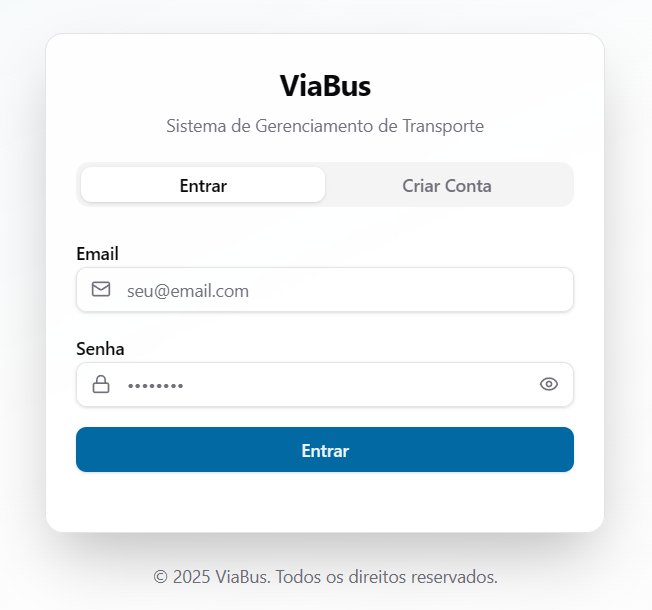
\includegraphics[width=0.6\textwidth]{imagens/tela-login.png}
  \caption{Tela de login do sistema ViaBus.}
  \label{fig:tela-login}
\end{figure}

\begin{figure}[H]
  \centering
  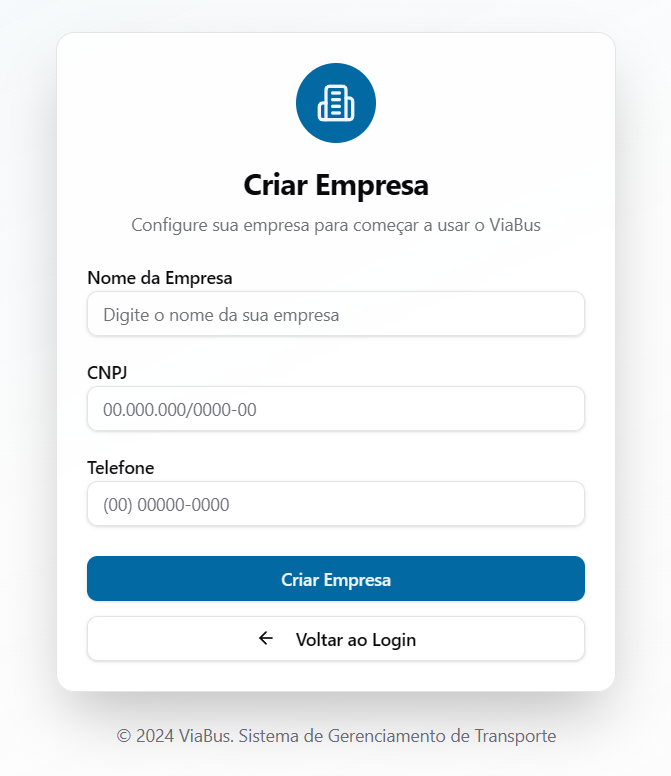
\includegraphics[width=0.6\textwidth]{imagens/criacao-empresa.png}
  \caption{Formulário de criação de empresa.}
  \label{fig:criacao-empresa}
\end{figure}

\subsubsection{Painel de Controle (Dashboard)}
Após o login, o gestor acessa o painel de controle (\textit{dashboard}), que foi concebido para atender ao requisito de \textbf{RF10} (visualizar rapidamente a ocupação e outras métricas). A interface, apresentada na Figura~\ref{fig:dashboard}, serve como uma central de comando visual para o gestor.

Nesta fase do protótipo, o \textit{layout} apresenta uma representação visual dos principais indicadores da operação. O \textit{design} foi projetado para, em futuras iterações, exibir cartões com dados consolidados e atualizados em tempo real, como o número de viagens, passagens vendidas, e o status de veículos e motoristas. O objetivo destes componentes é oferecer ao gestor um panorama instantâneo para a tomada de decisões estratégicas.

\begin{figure}[H]
  \centering
  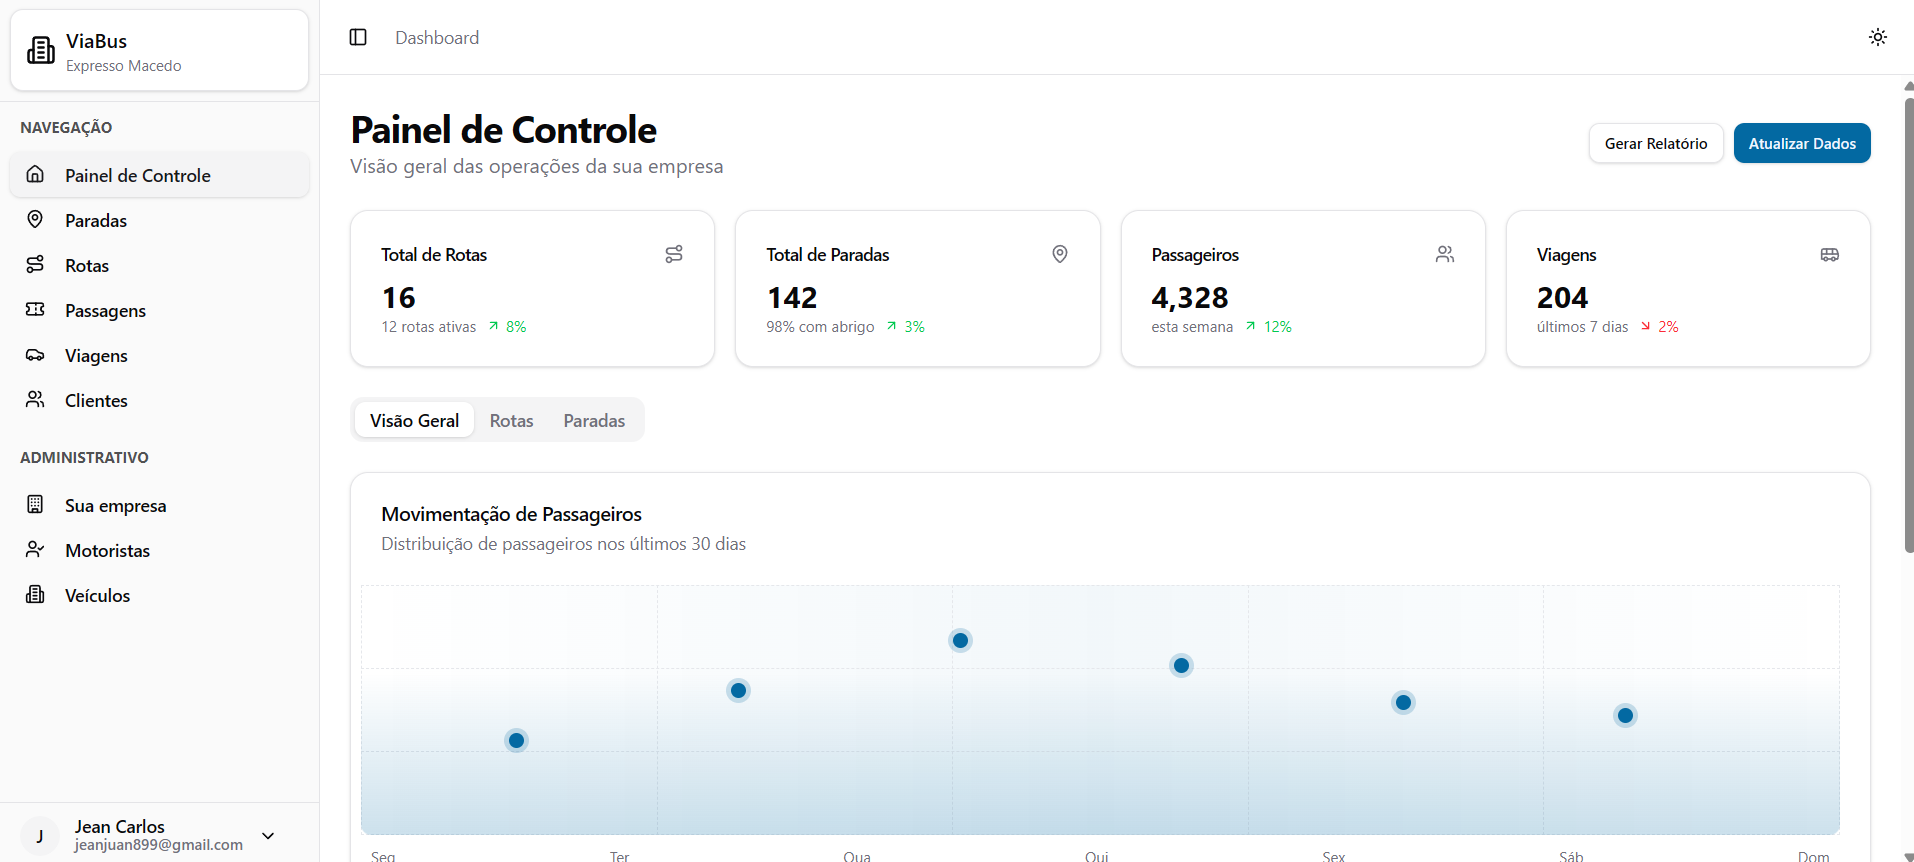
\includegraphics[width=1\textwidth]{imagens/dashboard.png}
  \caption{Painel de controle principal com métricas e navegação.}
  \label{fig:dashboard}
\end{figure}

\section{Gerenciamento de Recursos Operacionais}

Uma vez dentro do sistema, o gestor precisa configurar os recursos fundamentais de sua operação. Esta seção demonstra as interfaces criadas para o cadastro de paradas, rotas, veículos e motoristas.

\subsubsection{Gestão de Paradas e Rotas}
Para atender aos requisitos \textbf{RF03} (cadastro de pontos de parada) e \textbf{RF04} (organização de rotas), foram desenvolvidos módulos específicos. A Figura~\ref{fig:listagem-paradas} exibe a tela de listagem de paradas, enquanto a Figura~\ref{fig:formulario-parada} demonstra o formulário de cadastro, que integra um mapa interativo para facilitar a definição precisa da localização. Em seguida, na interface de criação de rotas (Figura~\ref{fig:criacao-rota}), o gestor pode selecionar essas paradas em uma sequência lógica para formar um itinerário.

\begin{figure}[H]
  \centering
  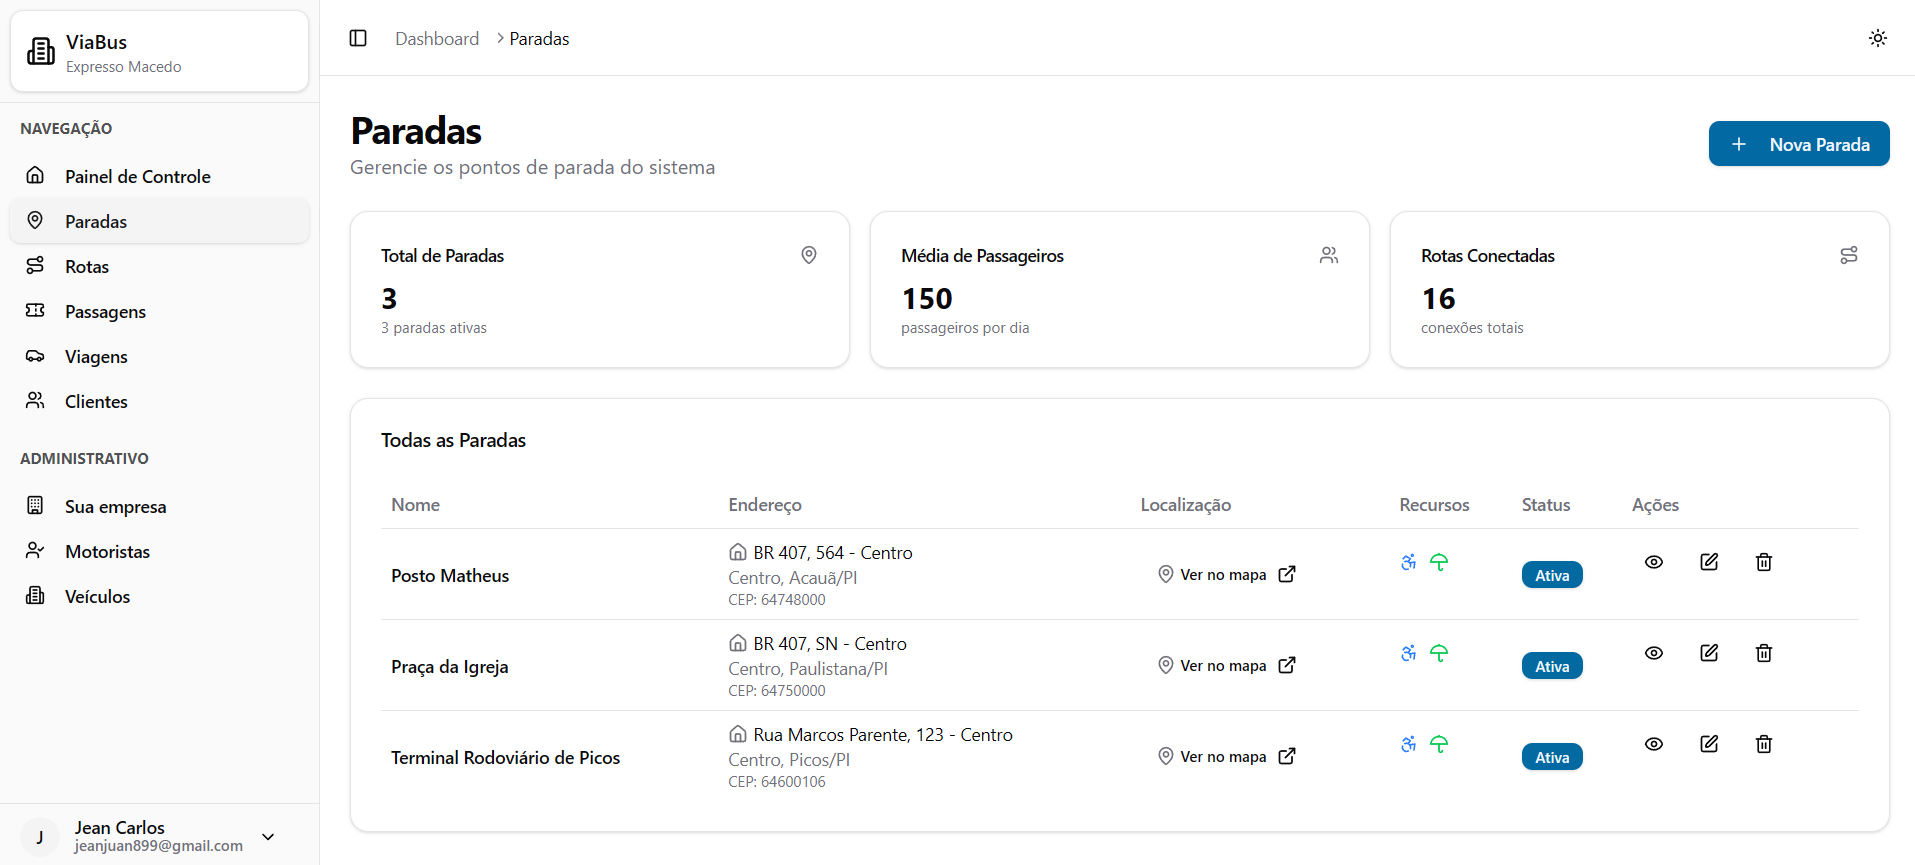
\includegraphics[width=1\textwidth]{imagens/listagem-paradas.png}
  \caption{Listagem de paradas com funcionalidades de busca e filtros.}
  \label{fig:listagem-paradas}
\end{figure}

\begin{figure}[H]
  \centering
  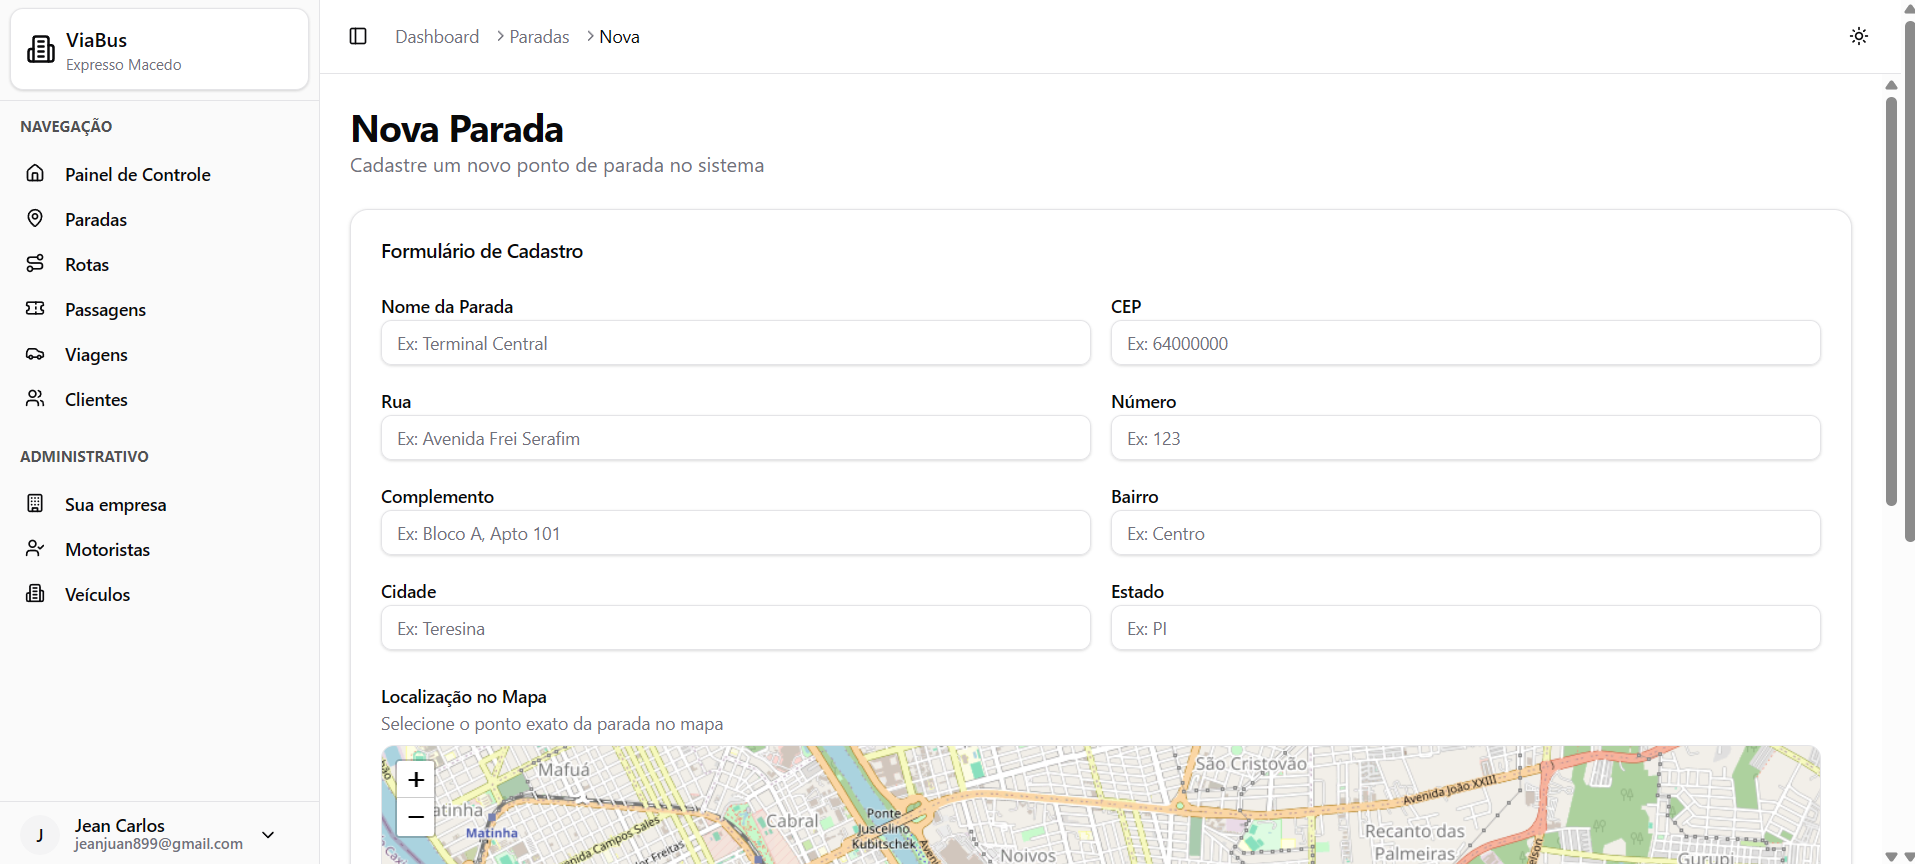
\includegraphics[width=1\textwidth]{imagens/formulario-parada.png}
  \caption{Formulário de cadastro de parada com mapa interativo.}
  \label{fig:formulario-parada}
\end{figure}

\begin{figure}[H]
  \centering
  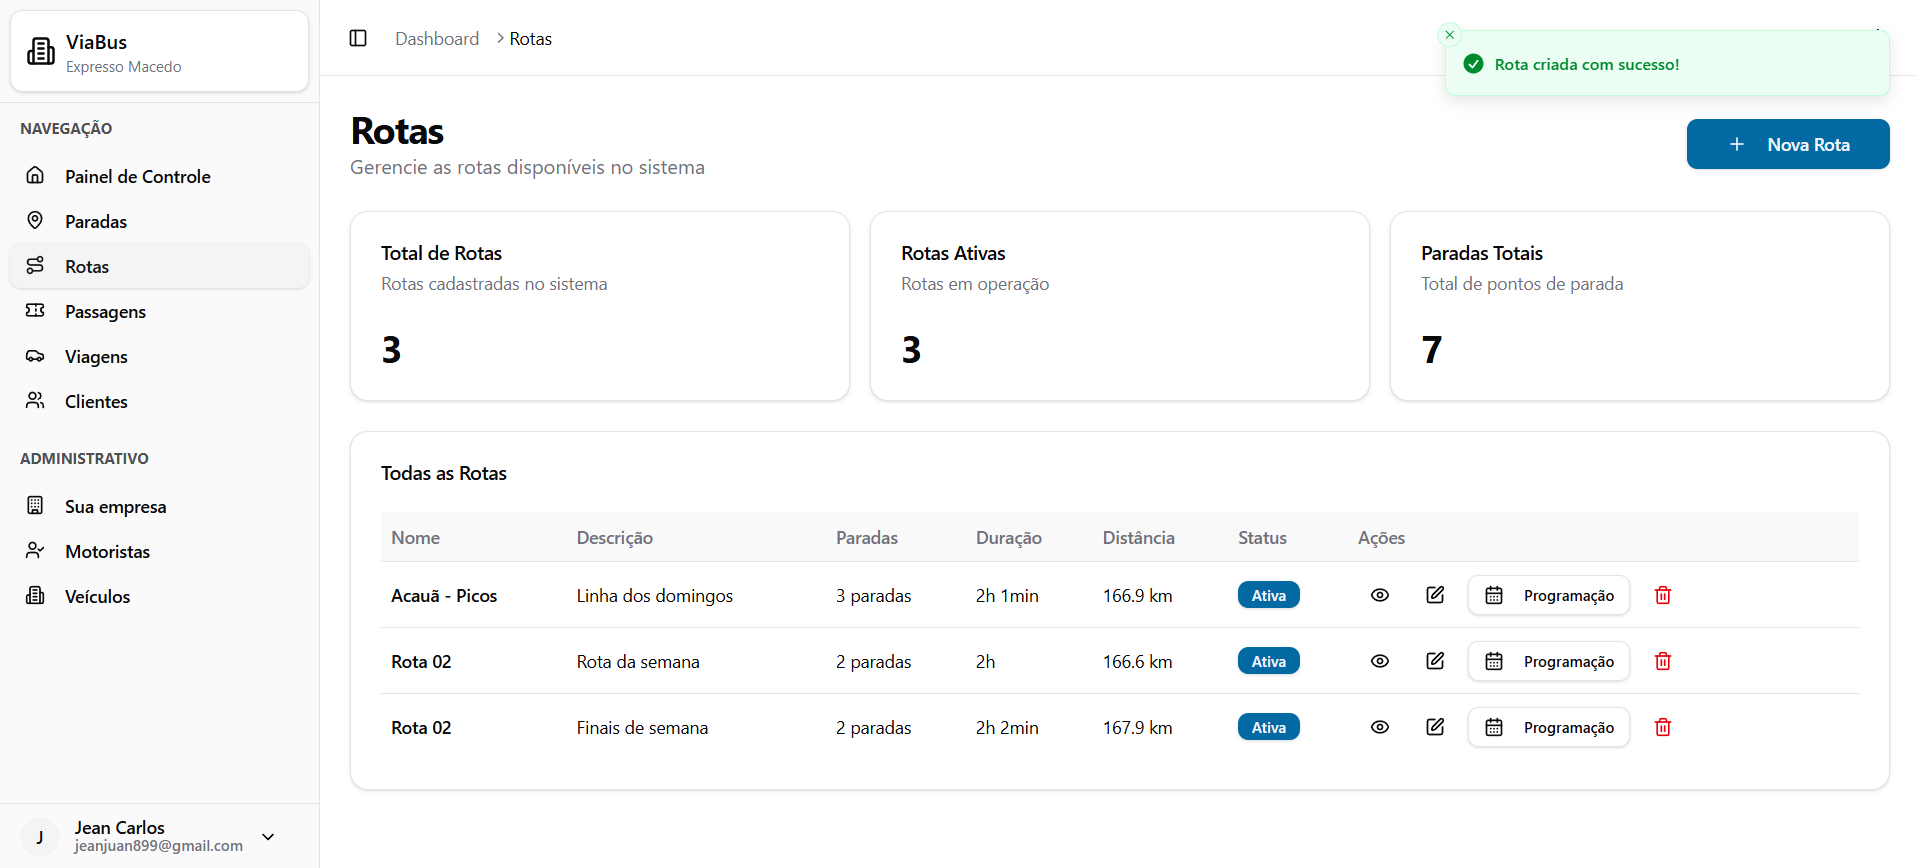
\includegraphics[width=1\textwidth]{imagens/tela-rotas.png}
  \caption{Listagem de rotas com funcionalidades de busca e filtros.}
  \label{fig:tela-rotas}
\end{figure}

\begin{figure}[H]
  \centering
  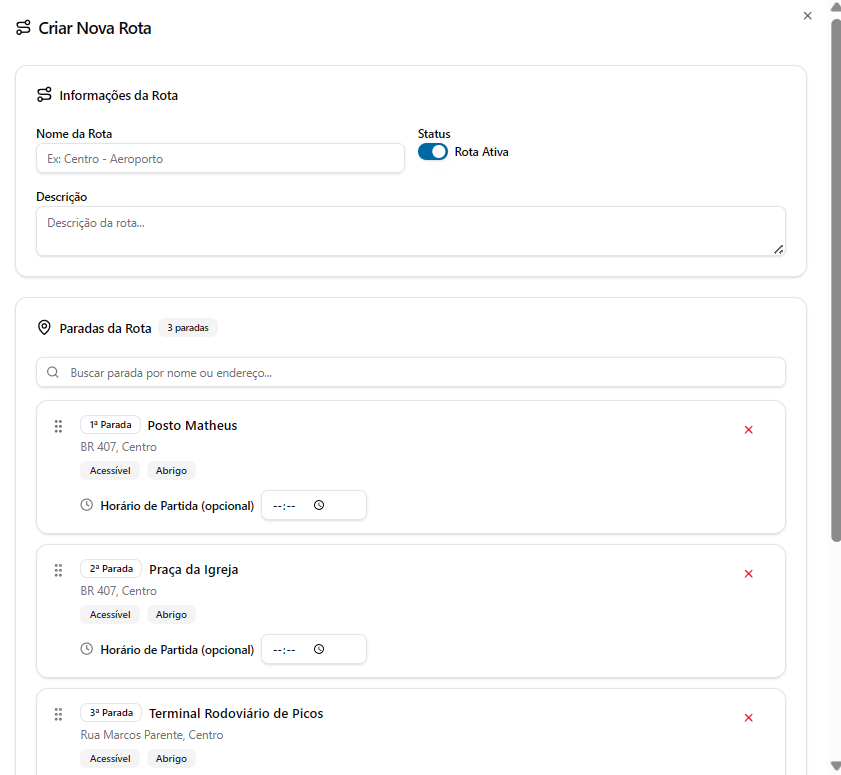
\includegraphics[width=0.7\textwidth]{imagens/criacao-rota.png}
  \caption{Interface de criação de rota com seleção de paradas.}
  \label{fig:criacao-rota}
\end{figure}

\subsubsection{Gestão da Frota e de Motoristas}
Atendendo aos requisitos \textbf{RF01} (gerenciar frota) e \textbf{RF02} (gerenciar motoristas), o sistema oferece interfaces dedicadas para o controle de veículos e condutores. As Figuras~\ref{fig:veiculos} e \ref{fig:motoristas} mostram as telas de listagem, onde é possível consultar informações detalhadas, verificar o status operacional de cada recurso e realizar ações de gerenciamento.

\begin{figure}[H]
  \centering
  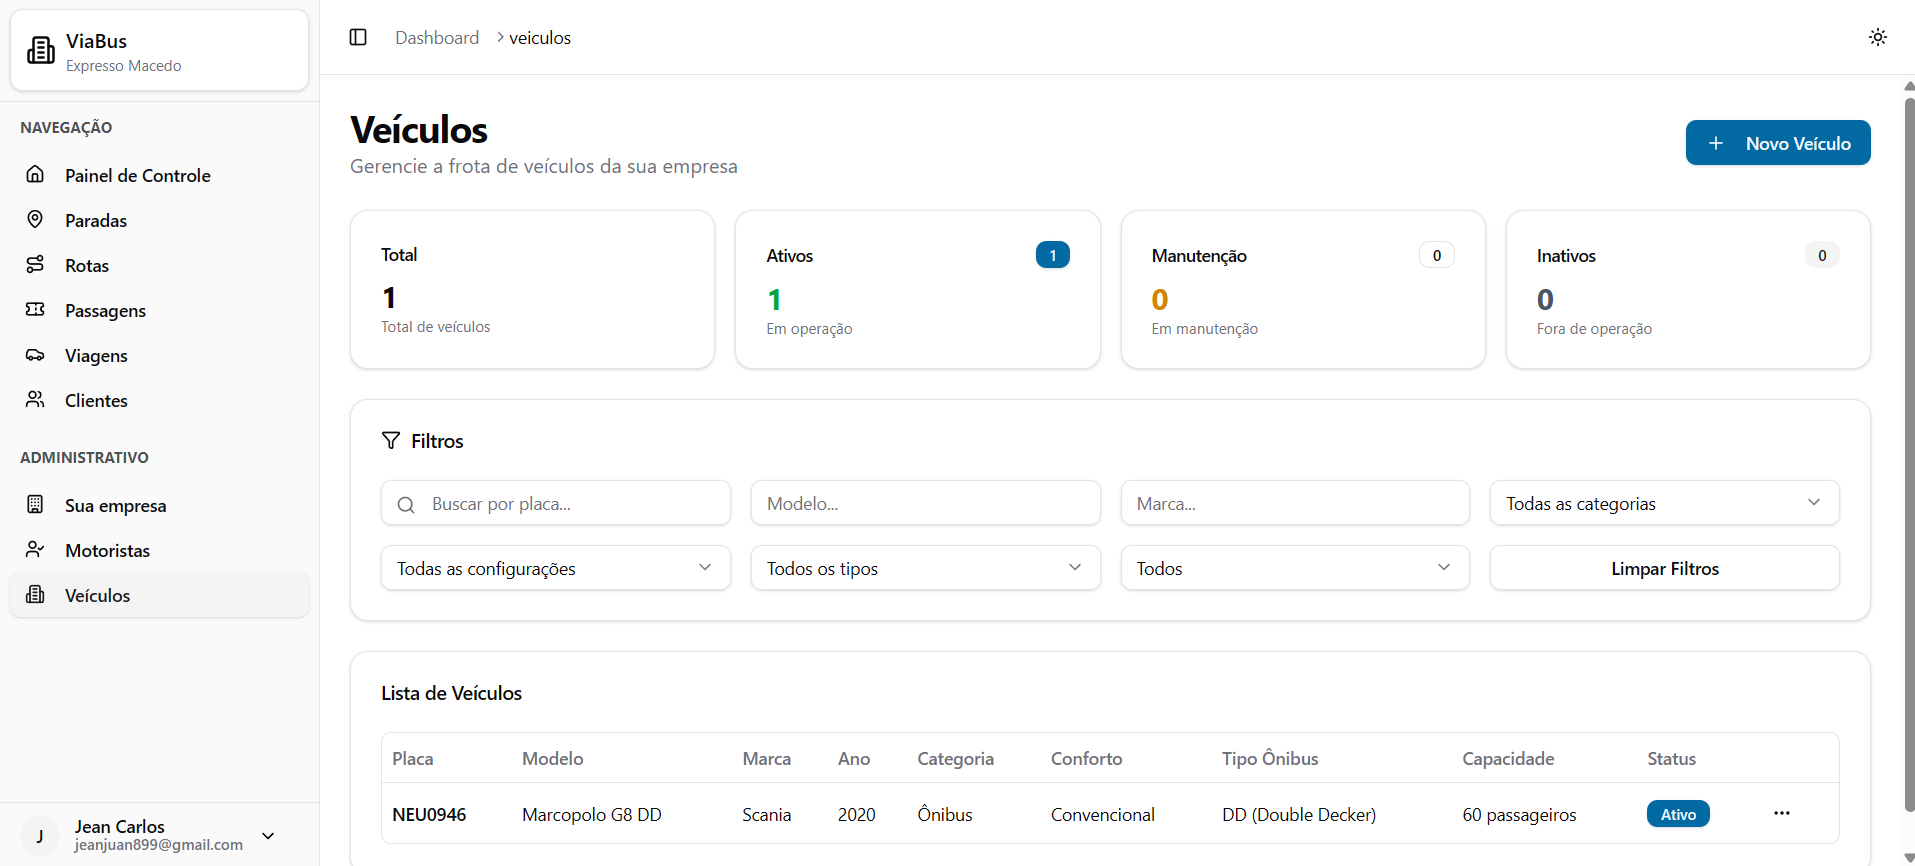
\includegraphics[width=1\textwidth]{imagens/veiculos.png}
  \caption{Listagem de veículos com status operacional.}
  \label{fig:veiculos}
\end{figure}

\begin{figure}[H]
  \centering
  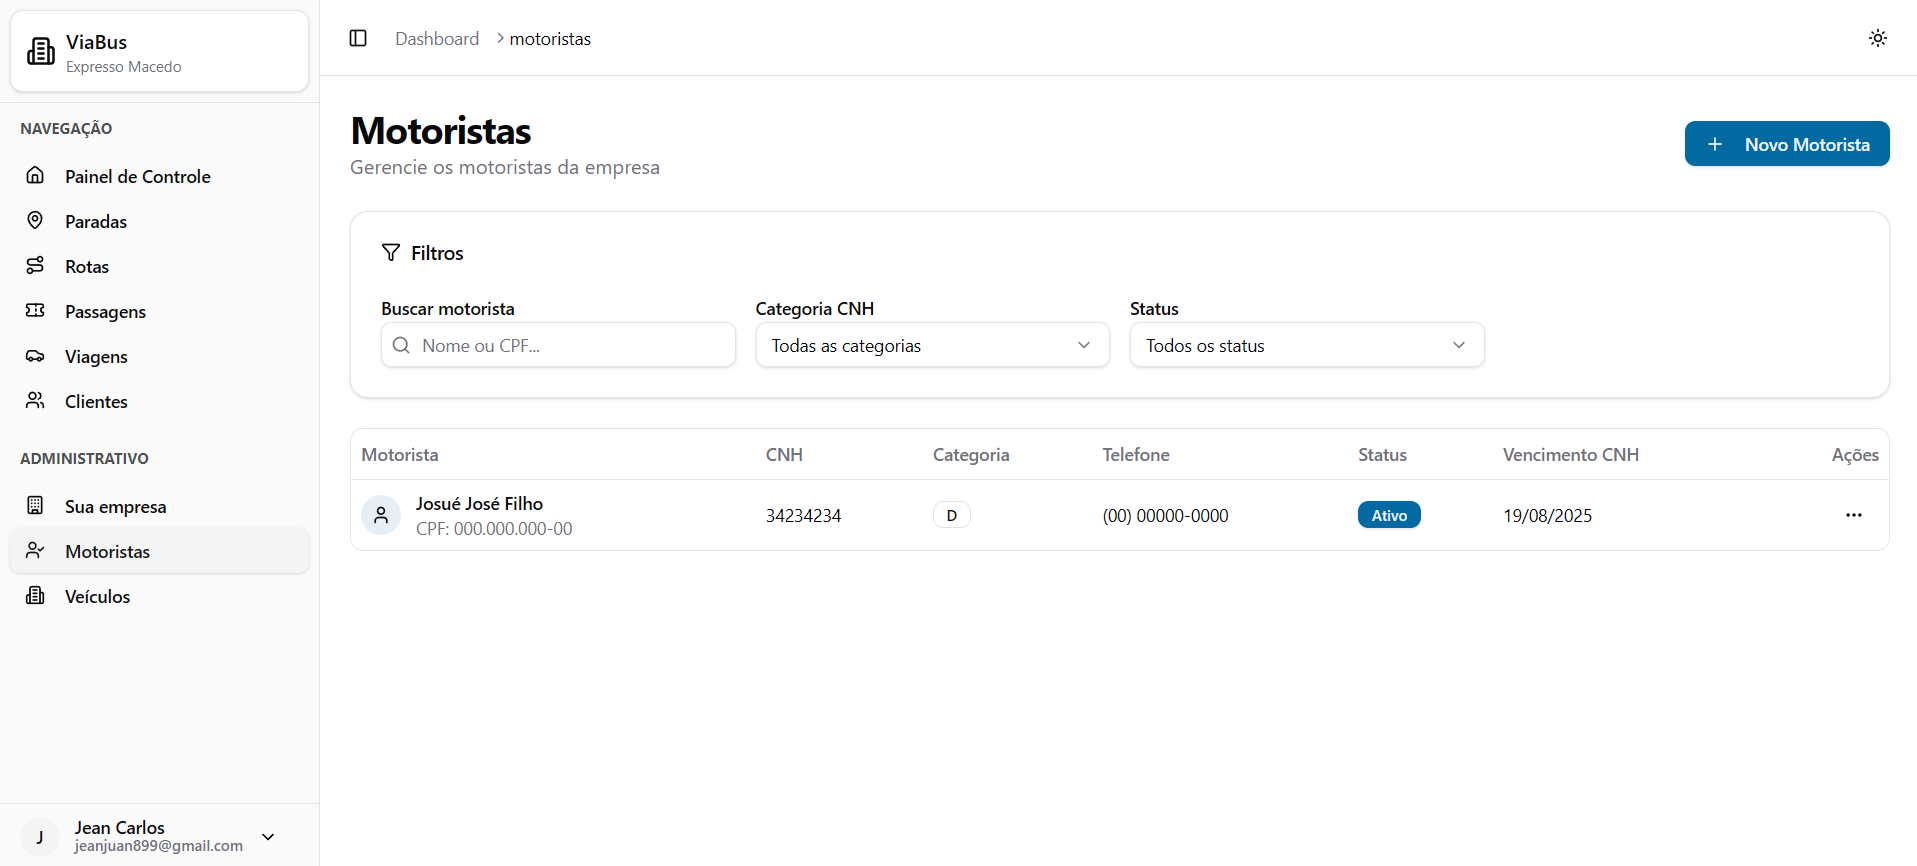
\includegraphics[width=1\textwidth]{imagens/motoristas.png}
  \caption{Interface de gerenciamento de motoristas.}
  \label{fig:motoristas}
\end{figure}

\section{Execução das Operações Diárias}

Com os recursos configurados, esta seção demonstra as funcionalidades centrais para a operação do dia a dia: o agendamento de viagens e a venda de passagens, que digitalizam o processo antes realizado em cadernos e aplicativos de mensagem.

\subsubsection{Agendamento de Viagens}
O requisito \textbf{RF05} (agendamento de viagens futuras) é materializado na interface da Figura~\ref{fig:agendamento-viagem}. Nela, o gestor pode criar uma nova viagem selecionando uma rota pré-definida e associando os recursos necessários, como o veículo e o motorista que realizarão o trajeto.

\begin{figure}[H]
  \centering
  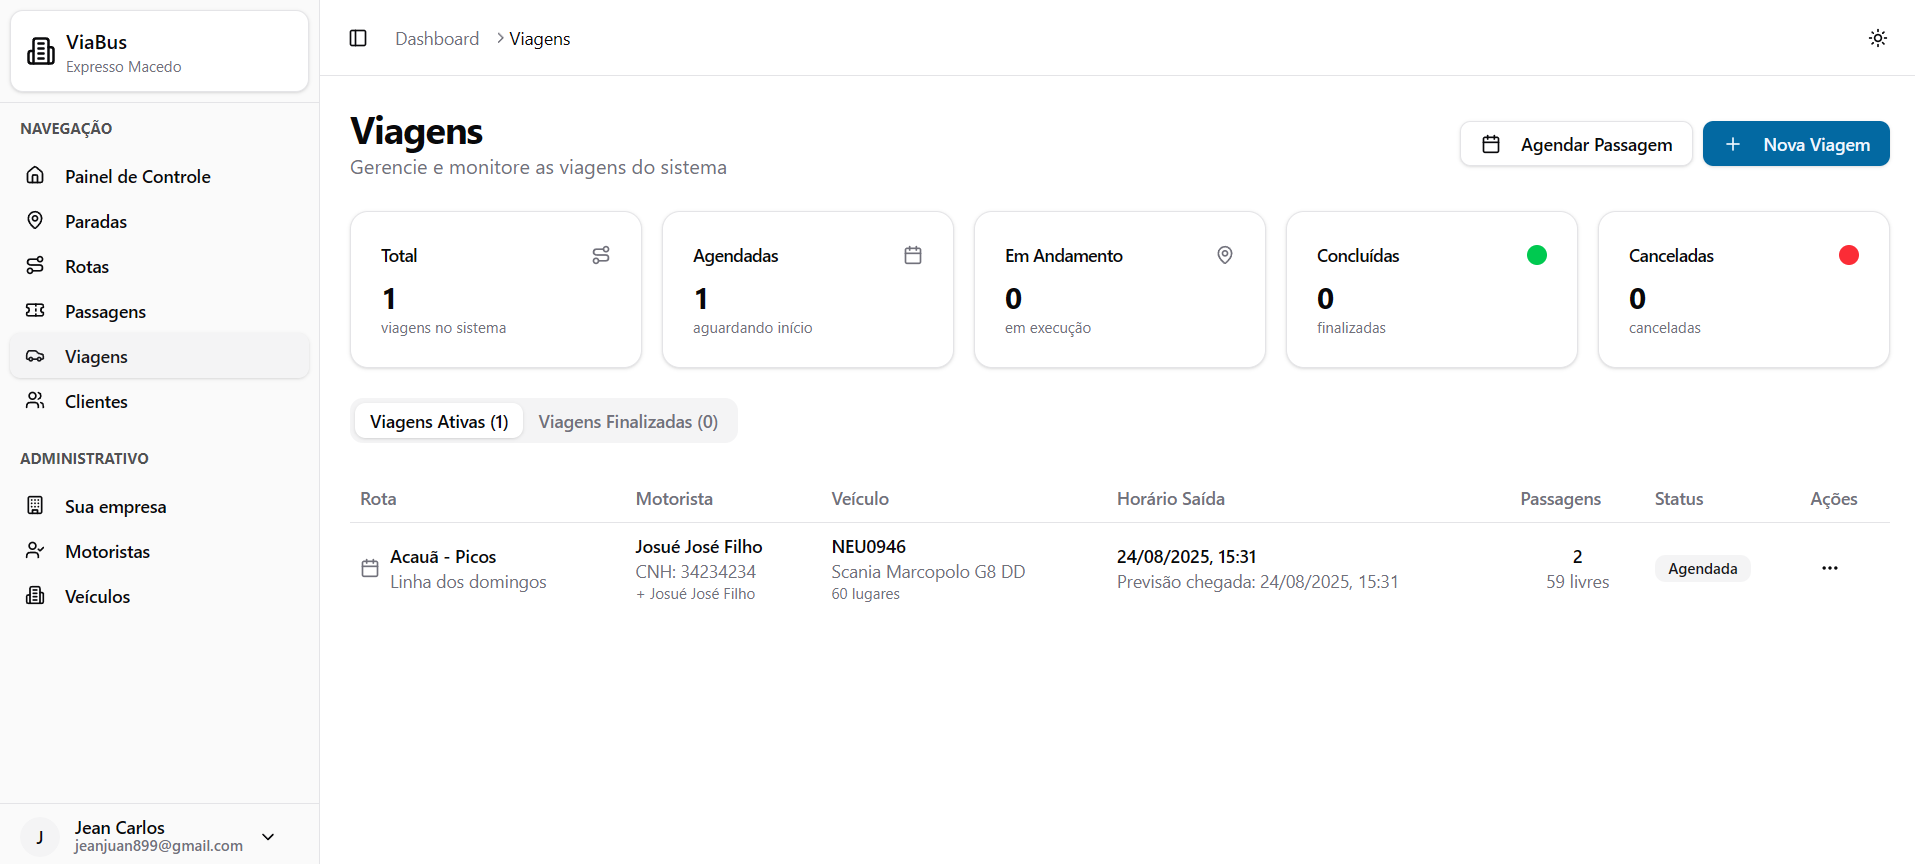
\includegraphics[width=1\textwidth]{imagens/agendamento-viagem.png}
  \caption{Processo de agendamento de viagem.}
  \label{fig:agendamento-viagem}
\end{figure}

\subsubsection{Assistente de Venda de Passagens}
O processo de venda de passagens foi projetado para ser rápido e à prova de erros, atendendo a um conjunto de requisitos essenciais. Para cumprir o \textbf{RF06} (venda rápida e guiada), foi implementado um assistente (\textit{wizard}) em cinco etapas. O fluxo se inicia com a seleção da rota e horário (Figuras~\ref{fig:wizard-rota} e \ref{fig:wizard-data}). Em seguida, são coletadas as informações do passageiro, conforme o \textbf{RF07} (Figura~\ref{fig:wizard-passageiro}), e selecionados os locais de embarque e desembarque (Figura~\ref{fig:wizard-locais}). Durante todo o processo, o sistema valida a disponibilidade de assentos em tempo real, satisfazendo o requisito crítico \textbf{RF08} (evitar overbooking). A etapa final (Figura~\ref{fig:wizard-confirmacao}) resume a venda e gera o bilhete, que pode ser usado para compor a lista de passageiros do \textbf{RF09}.

\begin{figure}[H]
  \centering
  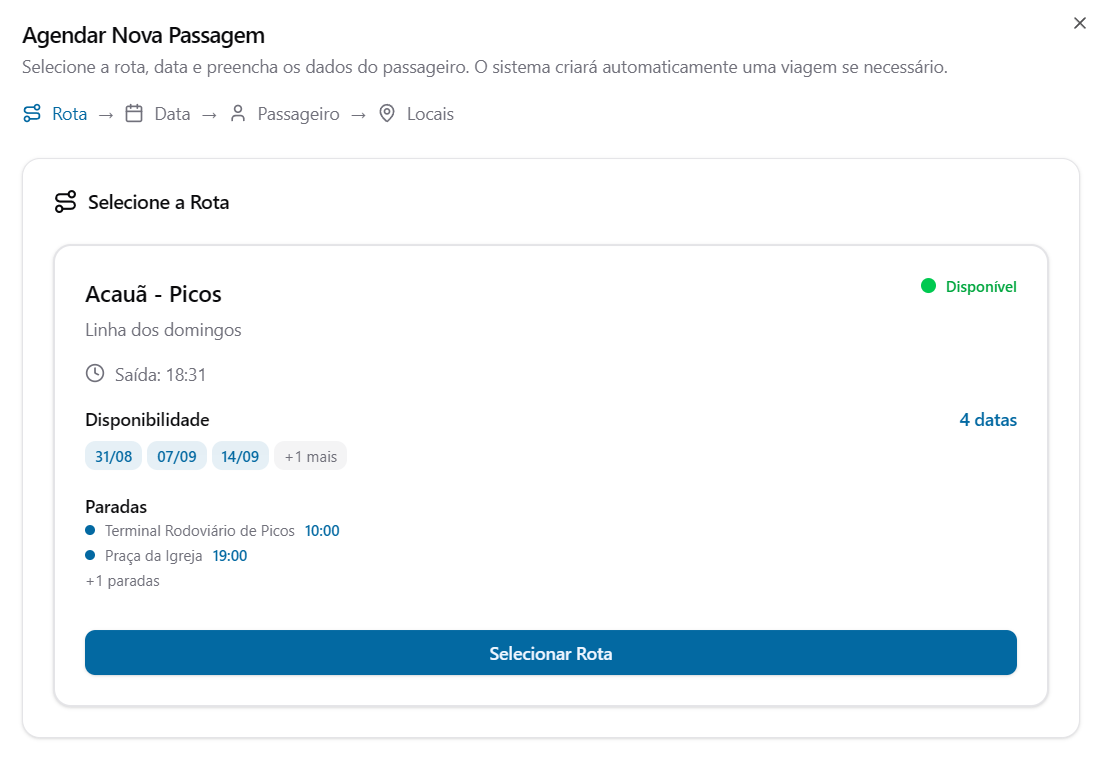
\includegraphics[width=0.8\textwidth]{imagens/wizard-rota.png}
  \caption{Seleção de rota no wizard de passagens.}
  \label{fig:wizard-rota}
\end{figure}

\begin{figure}[H]
  \centering
  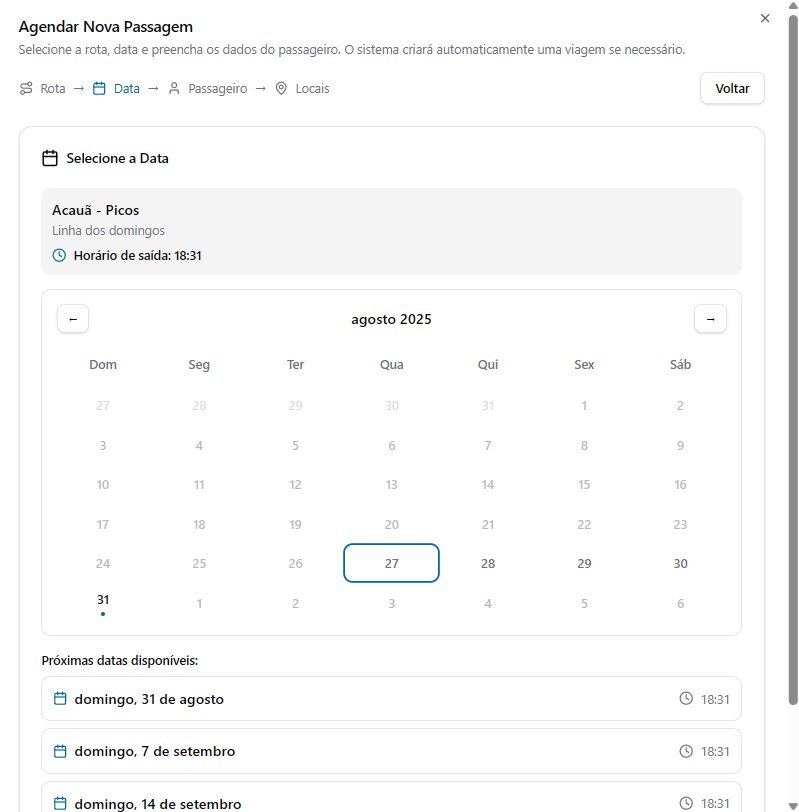
\includegraphics[width=0.6\textwidth]{imagens/wizard-data.png}
  \caption{Seleção de data e horário.}
  \label{fig:wizard-data}
\end{figure}

\begin{figure}[H]
  \centering
  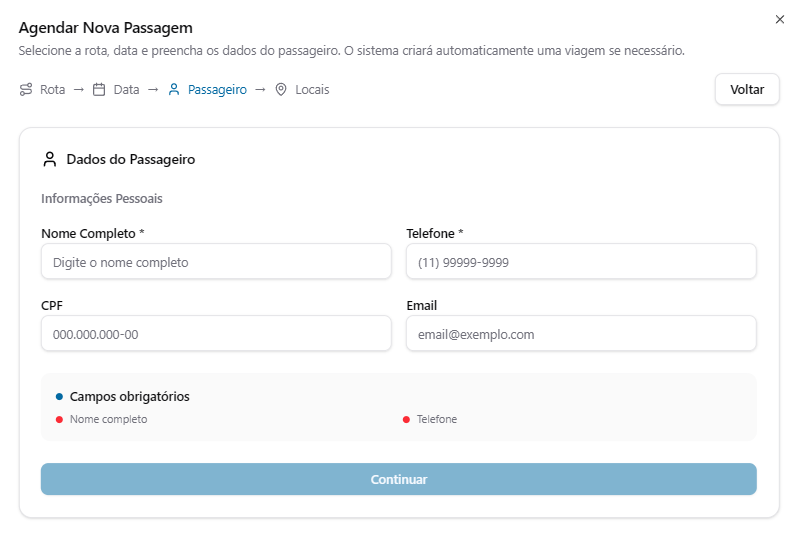
\includegraphics[width=0.8\textwidth]{imagens/wizard-passageiro.png}
  \caption{Cadastro de informações do passageiro.}
  \label{fig:wizard-passageiro}
\end{figure}

\begin{figure}[H]
  \centering
  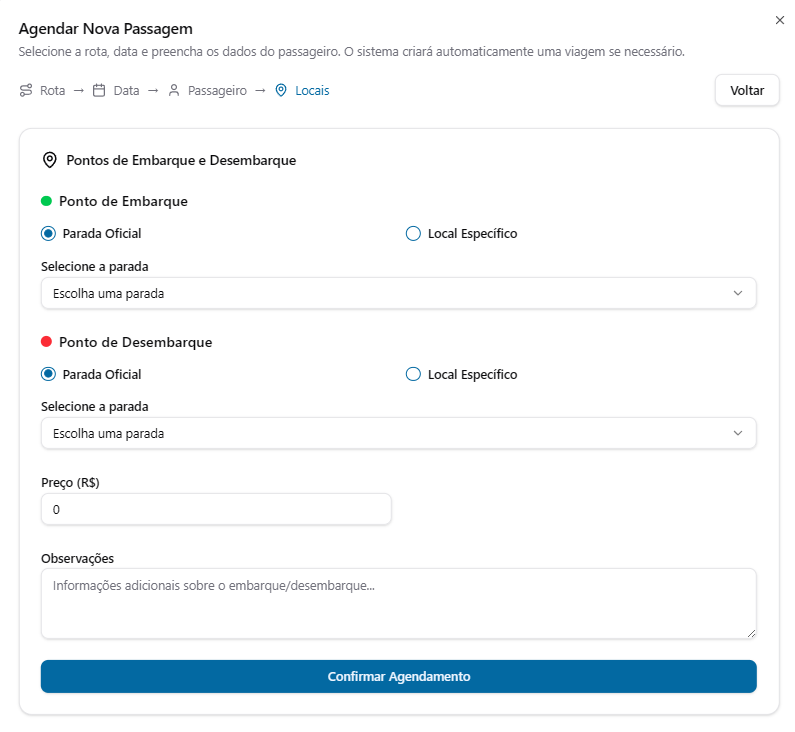
\includegraphics[width=0.7\textwidth]{imagens/wizard-locais.png}
  \caption{Seleção de locais de embarque e desembarque.}
  \label{fig:wizard-locais}
\end{figure}

\begin{figure}[H]
  \centering
  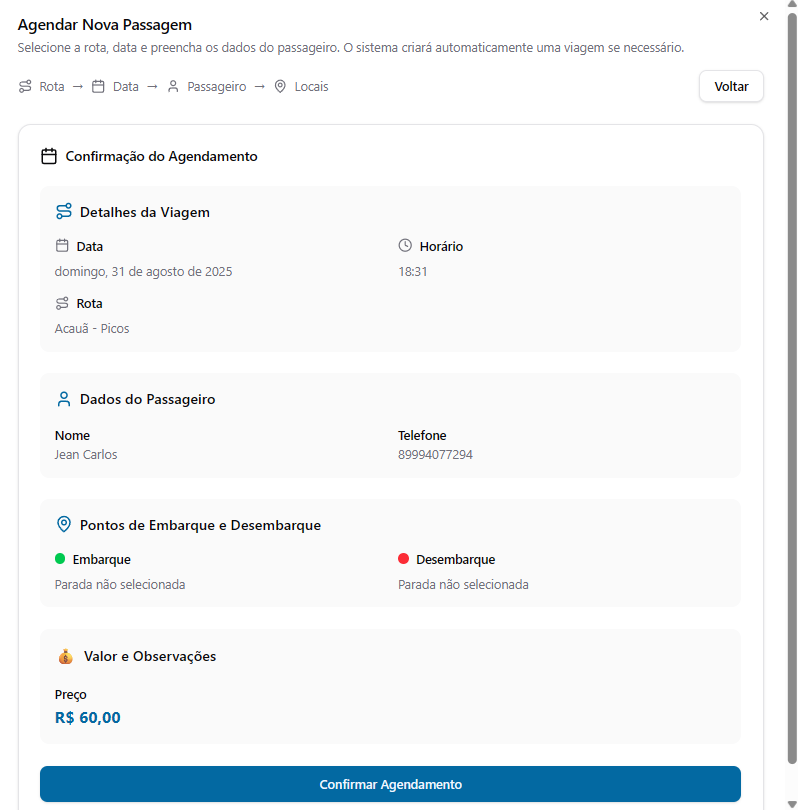
\includegraphics[width=0.7\textwidth]{imagens/wizard-confirmacao.png}
  \caption{Confirmação final e geração da passagem.}
  \label{fig:wizard-confirmacao}
\end{figure}